\chapter[Fundamentação Teórica]{Fundamentação Teórica} \label{c1}

  Este capítulo apresenta a base teórica para o entendimento do algoritmo a ser implementado. Nele, são explicados conceitos referentes a teoria musical, grafos e paradigmas de solução de problemas. Na seção sobre teoria musical, são abordados os tópicos de notação musical, intervalos, escalas e contrapontos. Na seção sobre grafos, são explicadas classificações para um grafo, o que são grafos direcionados acíclicos e tipos de travessia em grafos. Na seção sobre paradigmas de solução de problemas, são abordados dois paradigmas de solução de problema: busca completa e programação dinâmica.

  \section[Teoria Musical]{Teoria Musical}

    A música é a arte de combinar sons e silêncios. Segundo \citeonline{bohumil}, a música é constituída, principalmente, por melodia, harmonia, ritmo e contraponto. A melodia caracteriza-se por sons em ordem sucessiva, enquanto a harmonia caracteriza-se por sons em ordem simultânea. O ritmo é a ordem e proporção do sons de uma música. Já o contraponto é definido por meio de duas melodias dispostas simultaneamente.

    Os sons são parte fundamental da música. Cada som possui diversas características como altura (frequência do som que o torna mais grave ou mais agudo), duração, intensidade e timbre. Quando o som é regular (possui altura definida), ele pode ser expresso por meio de notação musical.

    \subsection[Notação Musical]{Notação Musical}

      As notas musicais são utilizadas para representar os sons de uma música. Há sete notas musicais -- usualmente nomeadas Dó, Ré, Mi, Fá, Sol, Lá, Si ou, respectivamente, C, D, E, F, G, A, B -- que podem variar de acordo com a oitava ou acidentes musicais empregados, para representação de tais modificações, elas são dispostas em uma pauta, conforme exemplificado na Figura \ref{pauta}.

      \begin{figure}[htb]
        \centering
        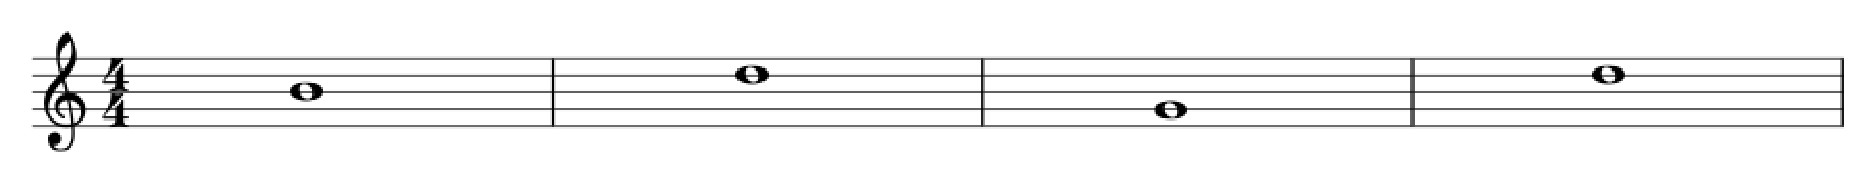
\includegraphics[scale=0.45]{figuras/pauta.eps}
        \caption{Pauta musical}
        \label{pauta}
      \end{figure}

      A pauta é utilizada para a representação de uma música, contendo linhas e espaços que definem a nota e em qual oitava está posicionada tendo como base a clave definida. Cada clave define uma nota específica e todas as outras notas da pauta são definidas a partir desta. Por exemplo, a clave de Sol é a mais comumente usada e define que a nota da linha 2 é o G4 (Sol da quarta oitava, Figura \ref{notas}).

      \begin{figure}[htb]
        \centering
        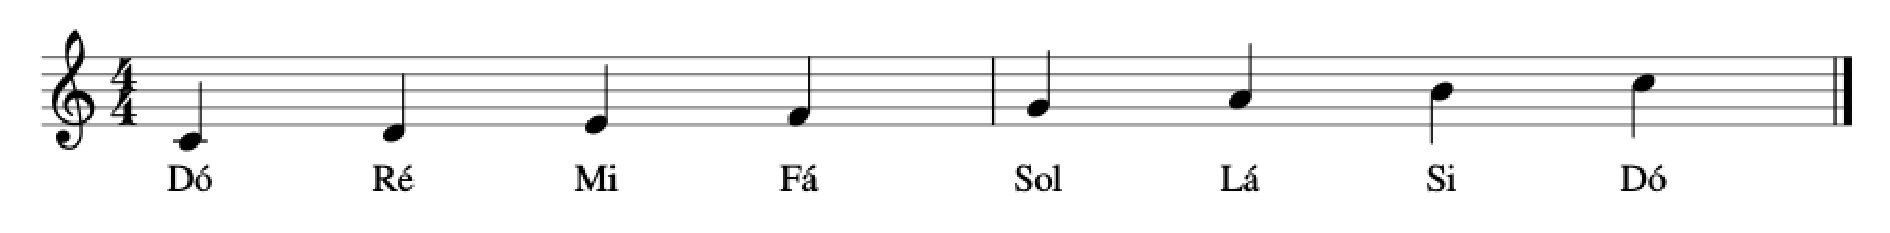
\includegraphics[scale=0.45]{figuras/notas.eps}
        \caption{Notas musicais na clave de Sol}
        \label{notas}
      \end{figure}

      % TODO: jeito certo de citar tabela
      Além da altura, cada som possui uma duração representada pela figura musical na pauta. No sistema atual, começa-se pela semibreve, que possui valor 1. A partir dela, a próxima subdivisão equivale à metade do tempo da anterior. Sendo assim, a mínima possui metade da duração da semibreve e possui valor 2, a semínima possui metade da duração da mínima e possui valor 4 e assim sucessivamente. As figuras, seus valores e durações estão representados na Tabela \ref{figurasmusicais}.

      \begin{table}[h]
      	\centering
        \caption{Figuras Musicais}
      	\begin{tabular}{cccc}
      		\toprule
      		\textbf{Nome} & \textbf{Figura} & \textbf{Valor} &
      		\textbf{Duração} \\
      		\midrule
      		Semibreve & \musSemibreve & 1 & 2 \musMinim \\
      		Mínima & \musMinim & 2 & $\nicefrac{1}{2}$ \musSemibreve{}  ou 2 \musQuarter \\
          Semínima & \musQuarter & 4 & $\nicefrac{1}{2}$ \musMinim{}  ou 2 \musCorchea \\
          Colcheia & \musCorchea & 8 & $\nicefrac{1}{2}$ \musQuarter{}  ou 2 \musSixteenth \\
      		Semicolcheia & \musSixteenth & 16 & $\nicefrac{1}{2}$ \musCorchea \\
      		\bottomrule
      	\end{tabular}
      	\label{figurasmusicais}
      \end{table}

      A duração em segundos de uma nota é definida pela sua figura e pelo andamento da música. O andamento define quantas notas de uma determinada figura de ritmo pode ser tocada em um espaço de tempo. Comumente, utiliza-se a quantidade de semínimas que podem ser tocadas durante um minuto para se definir o andamento de uma música.

      Em uma pauta, as figuras de ritmo são agrupadas em compassos. Cada compasso pode agrupar um determinado número de notas de acordo com sua estrutura, definida pela quantidade de figuras e a figura de ritmo usada como base. Por exemplo, um compasso 3/4 possui 3 como a quantidade de valores e 4 como a figura de ritmo, sendo assim, esse tipo de compasso é preenchido por três semínimas -- que possui valor 4. Desse modo, é possível também encaixar seis colcheias (que possui metade da duração de uma semínima) ou uma mínima e uma semínima em um compasso 3/4. Na música, a estrutura do compasso também define os tempos fortes e fracos da música. Em uma música 2/4, por exemplo, o primeiro tempo é forte (ou \textit{arsis}) e o segundo tempo é fraco (ou \textit{thesis}). Veja a Figura \ref{compassos}.

      \begin{figure}[htb]
        \centering
        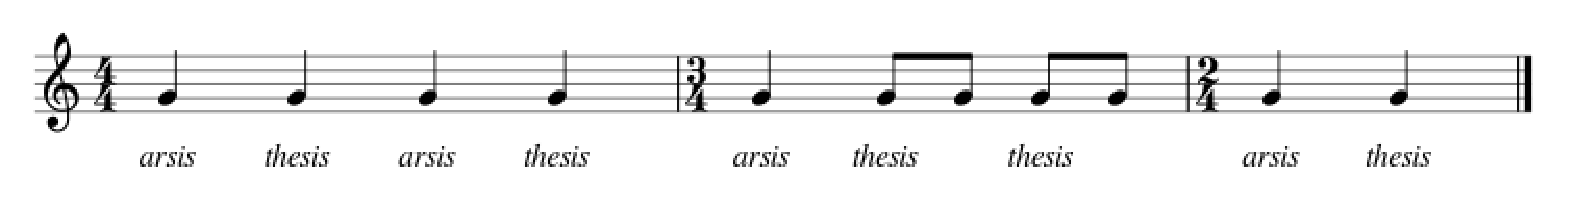
\includegraphics[scale=0.6]{figuras/compassos.eps}
        \caption{Exemplos de compasso e seus respectivos tempos fortes e fracos}
        \label{compassos}
      \end{figure}

      Outro elemento que pode ser representado na pauta são os acidentes musicais. Cada nota possui a distância relativa de um tom ou um semitom das notas adjacentes, como representado na Figura \ref{acidentes}. Essa distância calculada em tons e semitons também é utilizada para a definição de intervalos e pode ser modificada por meio de acidentes musicais.

      Existem dois tipos de acidentes musicais, o bemol (\fl) e o sustenido (\sh). O bemol abaixa a nota original em um semitom, como exemplo, o Fá e o Sol possuem um tom entre eles, porém, o Fá e o Sol bemol possuem um semitom entre eles. Já o sustenido aumenta a nota original em um semitom. Outras variações desses acidentes são o dobrado bemol, que abaixa a nota em um tom, o dobrado sustenido, que aumenta a nota em um tom e o bequadro, que retorna uma nota modificada ao seu valor original. Os símbolos de cada acidente estão representados na Figura \ref{acidentes}.

      \begin{figure}[htb]
        \centering
        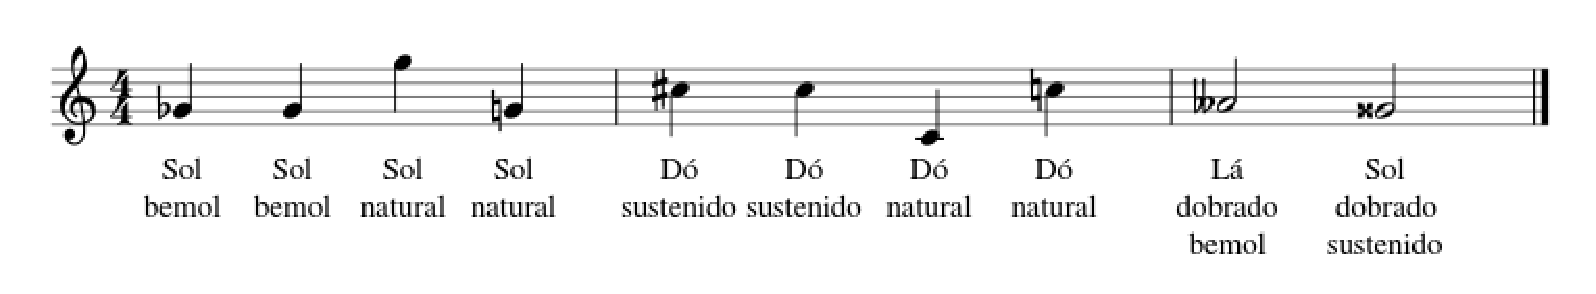
\includegraphics[scale=0.6]{figuras/acidentesmusicais.eps}
        \caption{Acidentes Musicais}
        \label{acidentes}
      \end{figure}

      Esses acidentes podem ser pontuais ou recorrentes durante uma música. Quando são pontuais, eles são expressos ao lado da nota que modificam, modificando também as notas de mesma altura naquele compasso. Quando são recorrentes, são representados no início da clave ou do primeiro compasso que modificam. Enquanto a representação pontual modifica apenas um único som em uma oitava específica, a representação no início modifica qualquer som daquela mesma nota, e a esse conjunto de acidentes representados no início da pauta dá-se o nome de armadura de clave. Veja a Figura \ref{armadura}.

      \begin{figure}[htb]
        \centering
        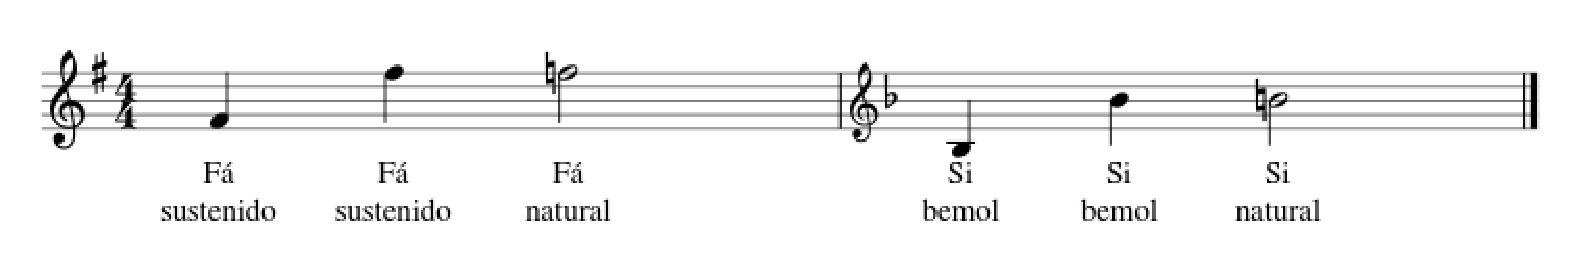
\includegraphics[scale=0.6]{figuras/armadura.eps}
        \caption{Armaduras de Clave}
        \label{armadura}
      \end{figure}

    \subsection[Intervalos]{Intervalos}

      A diferença de altura entre duas notas pode ser classificada por meio de intervalos. Os intervalos podem ser harmônicos (quando se compara duas notas simultâneas) e melódicos (quando se compara duas notas em sequência). Um intervalo melódico pode ser ascendente, se a primeira nota for mais grave que a segunda, e descendente, se a primeira nota for mais aguda que a segunda.

      Os intervalos também são classificados quantitativamente e qualitativamente. A classificação quantitativa de um intervalo tem como base a quantidade de notas entre as duas notas, incluindo-as e ignorando acidentes musicais. Por exemplo, a classificação quantitativa do intervalo entre o G4 (Sol na quarta oitava) e o E5 (Mi na quinta oitava) é sexta (6ª), que é a mesma que o intervalo entre G\sh4 (Sol sustenido na quarta oitava) e E\fl5 (Mi bemol na quinta oitava). Já a classificação qualitativa tem como base o número de tons e semitons entre as duas notas analisadas. Dependendo da quantidade de semitons, o intervalo pode ser justo (no caso de intervalos de primeira, quarta, quinta e oitava), maior, menor (no caso de intervalos de segunda, terça, sexta e sétima), aumentados ou diminutos.

      Cada intervalo pode ser classificado como consonante ou dissonante, uma classificação que define se o som provocado pelas duas notas soando seguidas ou em paralelo causam um efeito de repouso ou tensão, respectivamente. A classificação de um intervalo em relação ao seu efeito pode variar de acordo com a época ou estilo musical. Neste trabalho, será adotada a classificação correspondente às regras do contraponto modal do século XVI definidas por \citeonline{jeppesen}.

      \subsubsection[Intervalos Justos]{Intervalos Justos}

        % TODO: colocar abreviações nos primeiros exemplos de cada (1ªJ ou P1, 2ªM ou M2, etc)
        Os intervalos de primeira, quarta, quinta e oitava podem ser classificados como justos, dependendo da distância em semitons.

        Uma nota é a primeira justa (1ªJ ou P1\footnotemark \footnotetext{Sigla para \textit{perfect first}}) de outra se elas tiverem a mesma altura, ou seja, apenas uma nota entre elas e nenhum semitom de diferença, esse intervalo também é chamado de uníssono (Figura \ref{primeirajusta}).

        \begin{figure}[htb]
          \centering
          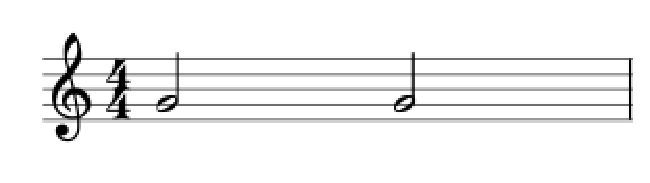
\includegraphics[scale=0.6]{figuras/primeirajusta.eps}
          \caption{Exemplo de Primeira Justa}
          \label{primeirajusta}
        \end{figure}


        A quarta justa (4ªJ ou P4) ocorre quando há quatro notas entre elas e a diferença é de dois tons e um semitom. Veja a Figura \ref{quartajusta}.

        \begin{figure}[htb]
          \centering
          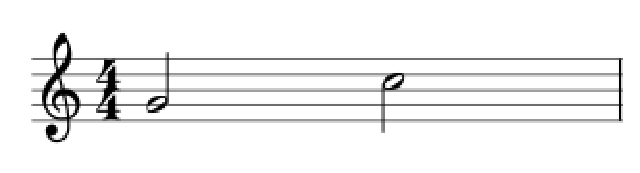
\includegraphics[scale=0.6]{figuras/quartajusta.eps}
          \caption{Exemplo de Quarta Justa}
          \label{quartajusta}
        \end{figure}

        A quinta justa (5ªJ ou P5) ocorre quando há cinco notas entre elas e a diferença é de três tons e um semitom. A Figura \ref{quintajusta} traz um exemplo de quinta justa.

        \begin{figure}[htb]
          \centering
          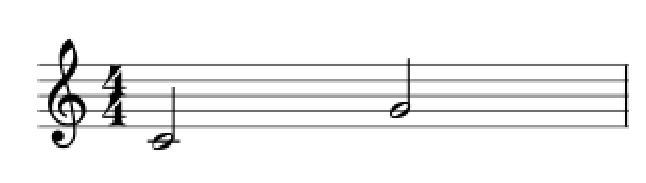
\includegraphics[scale=0.6]{figuras/quintajusta.eps}
          \caption{Exemplo de Quinta Justa}
          \label{quintajusta}
        \end{figure}

        A oitava justa (8ªJ ou P8) ocorre quando há oito notas entre elas e a diferença é de cinco tons e dois semitons (Figura \ref{oitavajusta}).

        \begin{figure}[htb]
          \centering
          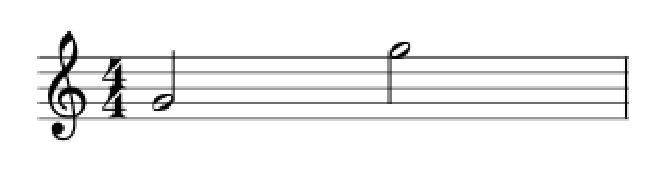
\includegraphics[scale=0.6]{figuras/oitavajusta.eps}
          \caption{Exemplo de Oitava Justa}
          \label{oitavajusta}
        \end{figure}

        Dentre os intervalos justos, todos, exceto a quarta justa, são considerados consonâncias perfeitas. Vale ressaltar que, segundo \citeonline{bohumil}, a quarta justa é considerada um intervalo consonante na música contemporânea.

      \subsubsection[Intervalos Maiores e Menores]{Intervalos Maiores e Menores}

        Os intervalos de segunda, terça, sexta e sétima podem ser classificados como maiores ou menores, dependendo da distância em semitons.

        A segunda ocorre quando há duas notas entre elas. A segunda menor (2ªm ou m2) ocorre quando a diferença é de um semitom, já a segunda maior (2ªM ou M2) possui uma diferença de um tom. Veja a Figura \ref{segundas}.

        \begin{figure}[htb]
          \centering
          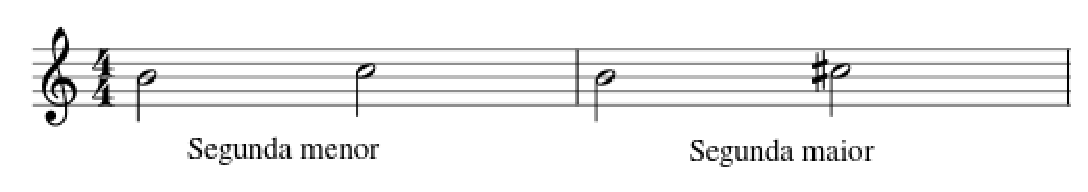
\includegraphics[scale=0.8]{figuras/segundas.eps}
          \caption{Exemplos de Segunda Menor e Segunda Maior}
          \label{segundas}
        \end{figure}


        A terça ocorre quando há três notas entre elas. A terça menor (3ªm ou m3) ocorre quando a diferença é de um tom e um semitom, já a terça maior (3ªM ou M3) possui uma diferença de dois tons (Figura \ref{tercas}).

        \begin{figure}[htb]
          \centering
          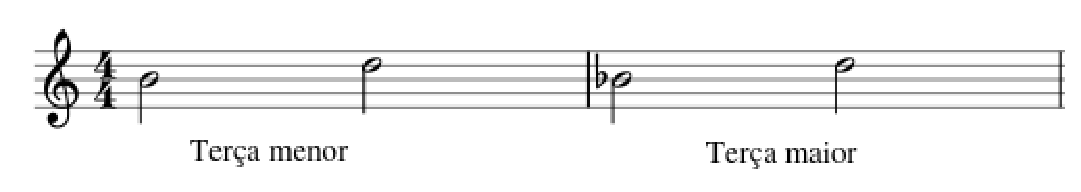
\includegraphics[scale=0.8]{figuras/tercas.eps}
          \caption{Exemplos de Terça Menor e Terça Maior}
          \label{tercas}
        \end{figure}

        A sexta ocorre quando há seis notas entre elas. A sexta menor (6ªm ou m6) ocorre quando a diferença é de três tons e dois semitons, já a sexta maior (6ªM ou M6) possui uma diferença de quatro tons e um semitom. Veja a Figura \ref{sextas}.

        \begin{figure}[htb]
          \centering
          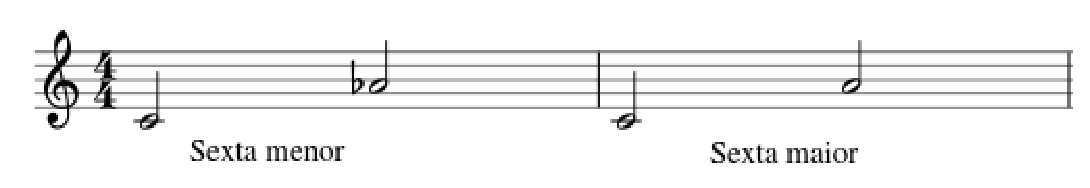
\includegraphics[scale=0.8]{figuras/sextas.eps}
          \caption{Exemplos de Sexta Menor e Sexta Maior}
          \label{sextas}
        \end{figure}

        A sétima ocorre quando há sete notas entre elas. A sétima menor (7ªm ou m7) ocorre quando a diferença é de quatro tons e dois semitons, já a sétima maior (7ªM ou M7) possui uma diferença de cinco tons e um semitom (Figura \ref{setimas}).

        \begin{figure}[htb]
          \centering
          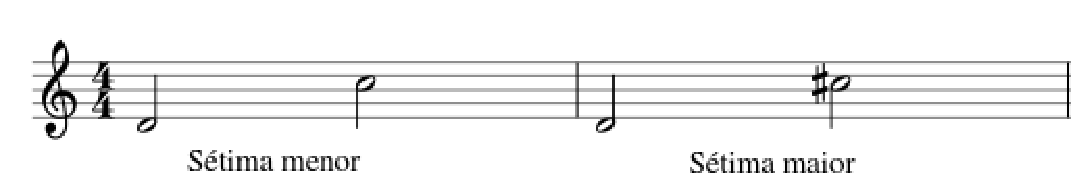
\includegraphics[scale=0.8]{figuras/setimas.eps}
          \caption{Exemplos de Sétima Menor e Sétima Maior}
          \label{setimas}
        \end{figure}

        Os intervalos de terça maior e menor e sexta maior e menor são classificados como consonâncias imperfeitas, enquanto os intervalos de segunda maior e menor e sétima maior e menor são classificados como dissonâncias.

      \subsubsection[Intervalos Aumentados e Diminutos]{Intervalos Aumentados e Diminutos}

        Se a distância em semitons das duas notas do intervalo não identificá-lo como justo, maior ou menor, ele será classificado como aumentado ou diminuto.

        Intervalos aumentados possuem mais semitons que os intervalos justos ou maiores. Se o intervalo possuir um semitom a mais, ele é chamado de aumentado, se forem dois semitons a mais, é chamado de superaumentado, se forem três semitons a mais, é chamado de três vezes aumentado e assim sucessivamente, até os maiores intervalos possíveis que são os cinco vezes aumentados. Na Figura \ref{aumentadas}, há exemplos de quarta aumentada (4ªA ou A4), quarta superaumentada (4ªSA ou SA4\footnotemark \footnotetext{Notação utilizada no código para intervalos superaumentados}) e quarta 3x aumentada (4ª3xA ou 3xA4\footnotemark \footnotetext{Notação utilizada no código para intervalos 3x, 4x e 5x aumentados}).

        \begin{figure}[htb]
          \centering
          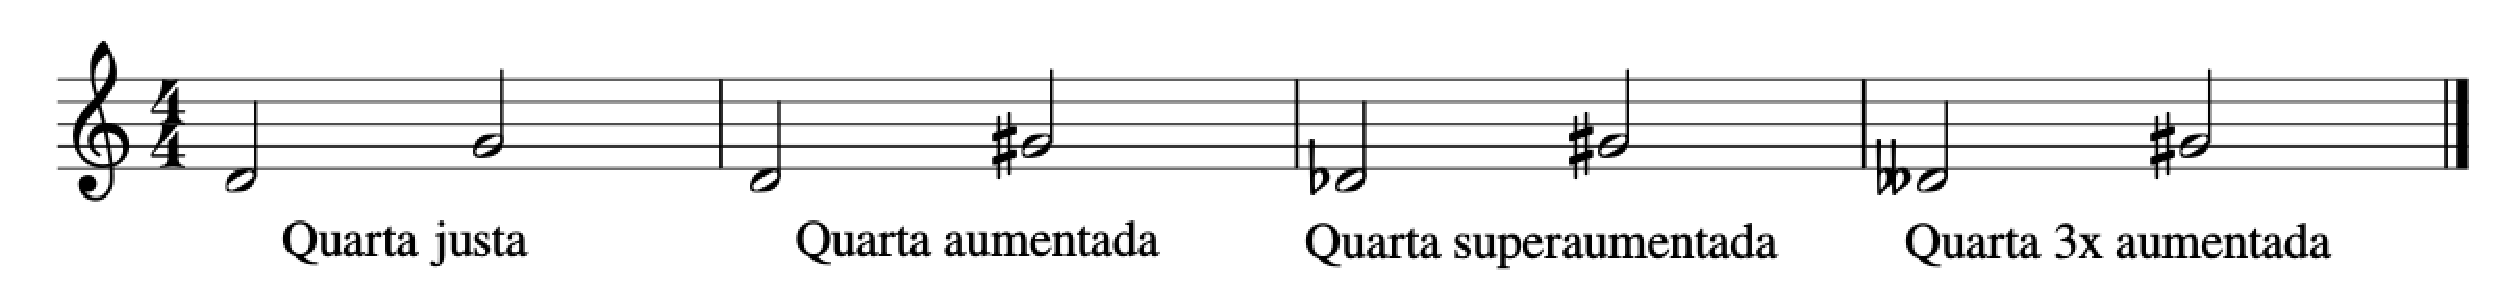
\includegraphics[scale=0.4]{figuras/aumentadas.eps}
          \caption{Exemplos de Intervalos Aumentados}
          \label{aumentadas}
        \end{figure}

        Intervalos diminutos possuem menos semitons que os intervalos justos ou menores. Se o intervalo possuir um semitom a menos, ele é chamado de diminutos, se forem dois semitons a menos, é chamado de superdiminuto, se forem três semitons a menos, é chamado de três vezes diminuto e assim sucessivamente, até os menores intervalos possíveis que são os cinco vezes diminutos. Na Figura \ref{diminutas}, há exemplos de sexta diminuta (6ªd ou d6), sexta superaumentada (6ªsd ou sd6\footnotemark \footnotetext{Notação utilizada no código para intervalos superdiminutos}) e sexta 3x aumentada (6ª3xd ou 3xd6\footnotemark \footnotetext{Notação utilizada no código para intervalos 3x, 4x e 5x diminutos}).

        \begin{figure}[htb]
          \centering
          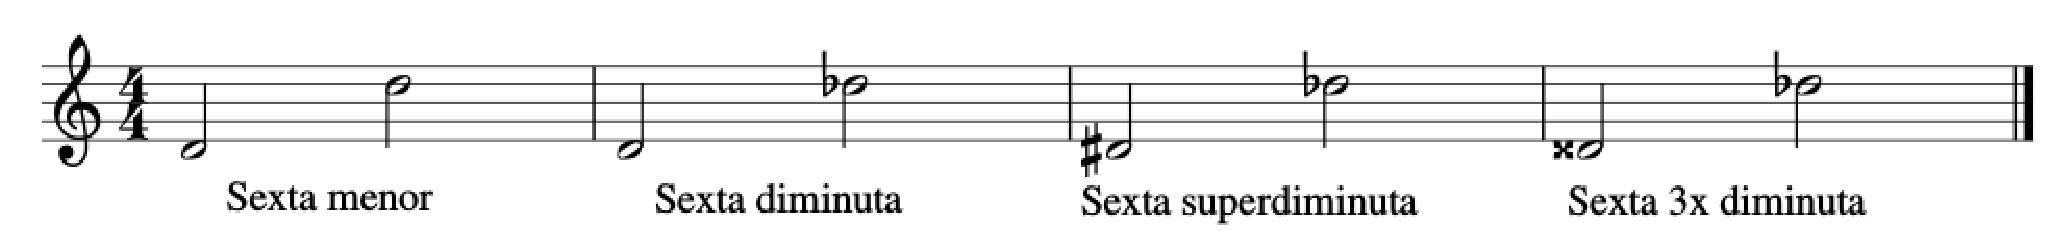
\includegraphics[scale=0.5]{figuras/diminutas.eps}
          \caption{Exemplos de Intervalos Diminutos}
          \label{diminutas}
        \end{figure}


        Os intervalos aumentados e diminutos são classificados como consonantes e dissonantes de acordo com os intervalos justos, maiores e menores que possuem a mesma distância em semitons, por exemplo, o intervalo de quarta superaumentada é considerado consonante pois possui a mesma distância em semitons que a quinta justa, embora sua classificação quantitativa seja a mesma que a quarta justa, classificada como dissonância. Por causa disso, os intervalos aumentados e diminutos são considerados dissonâncias condicionais.

      \subsubsection[Intervalos Compostos]{Intervalos Compostos}

        Se um intervalo ultrapassar a oitava justa, quantitativa ou qualitativamente, ele é considerado composto. Intervalos compostos tem sua classificação definida de acordo com seus correspondentes simples. Para classificar um intervalo composto, divide-se o valor quantitativo por 7 e o resto é utilizado para definir seu equivalente simples, por exemplo, uma 15ª corresponde a uma 1ª.

        Para a análise quantitativa, divide-se o valor de semitons por 12 e o resto é utilizado para definir se ele é justo, maior, menor, diminuto ou aumentado, por exemplo uma 10ª com uma diferença de 16 semitons é equivalente a uma 3ª com 4 semitons, sendo uma 3ª maior, logo, o intervalo analisado é uma 10ª maior.

        Os intervalos compostos são, basicamente, seus equivalentes simples somados a oitavas justas, como exemplificado na Figura \ref{compostos}. O intervalo de oitava aumentada é considerado composto e é equivalente ao intervalo de primeira aumentada.

        \begin{figure}[htb]
          \centering
          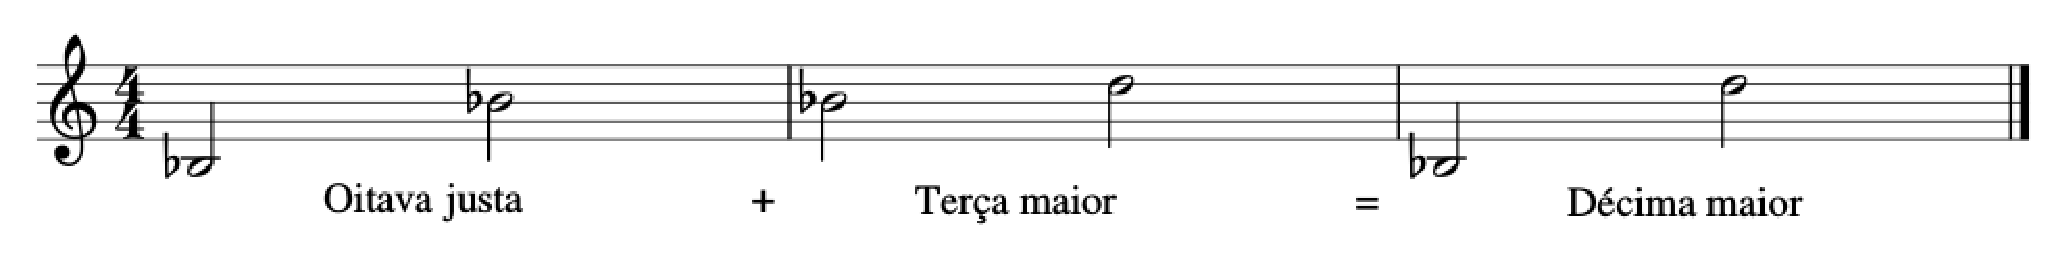
\includegraphics[scale=0.5]{figuras/compostos.eps}
          \caption{Exemplo de Intervalo Composto}
          \label{compostos}
        \end{figure}


    \subsection[Escalas]{Escalas}

      Segundo Med, escala é o conjunto de notas disponíveis em um sistema musical. As notas presentes em uma escala possuem intervalos específicos entre si. As escalas podem ser classificadas quanto ao número de notas, sendo as mais conhecidas a pentatônica (cinco notas), a hexacordal (seis notas), a heptatônica (sete notas) e a cromática (doze notas). A escala cromática, por exemplo, possui todas as dozes notas (com e sem acidentes) de uma oitava, tendo intervalos de segunda menor ou primeira aumentada entre elas (Figura \ref{cromatica}).

      \begin{figure}[htb]
        \centering
        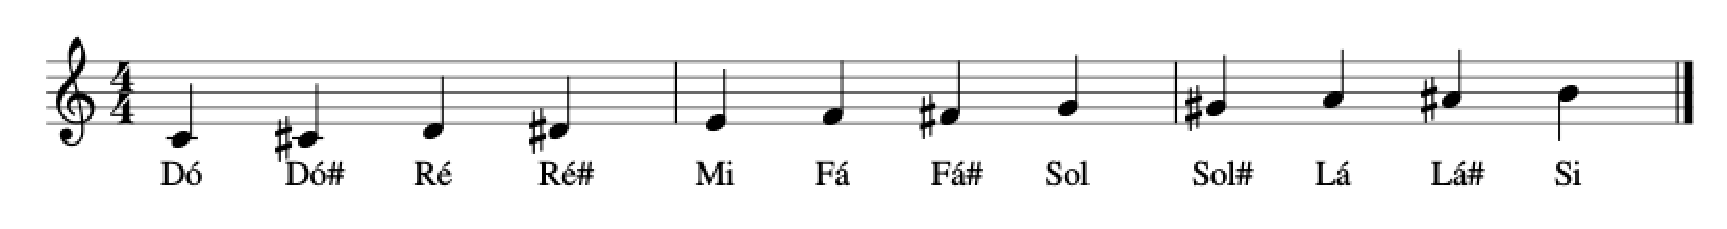
\includegraphics[scale=0.5]{figuras/cromatica.eps}
        \caption{Escala Cromática}
        \label{cromatica}
      \end{figure}

      % TODO: como citar figura?
      Outra classificação é quanto à utilização, as mais conhecidas são as escalas classificadas como diatônicas, que possuem oito notas, sete distintas e a última sendo a primeira uma oitava acima, possuindo intervalos de segunda maior ou menor entre elas. Em uma escala diatônica, pode-se definir quais notas fazem parte dela observando a armadura de clave presente na partitura. Por exemplo, na escala representada na figura \ref{escaladiatonica}, há uma armadura de sustenindo em F (Fá) e em C (Dó), logo, a escala possui as seguintes notas: D, E, F\sh, G, A, B e C\sh. Músicas compostas nessa escala não podem possuir notas como A\fl, B\sh{} ou C, a não ser em caso de acidentes pontuais, definidos pelo compositor. Cada nota de uma escala diatônica possui um grau (que varia de um a sete) e um nome específicos. A principal nota é a de grau I, chamada tônica. Ela dá nome à escala e a inicia, tendo todas as outras notas definidas a partir dela.

      \begin{figure}[htb]
        \centering
        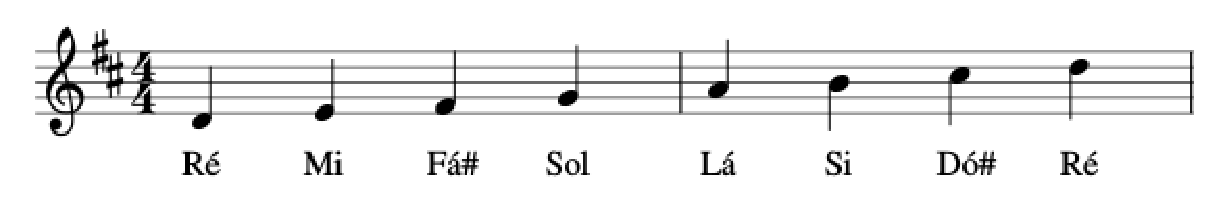
\includegraphics[scale=0.6]{figuras/escalaremaior.eps}
        \caption{Exemplo de Escala Diatônica}
        \label{escaladiatonica}
      \end{figure}

      \subsubsection[Escalas Maiores]{Escalas Maiores}

        As escalas diatõnicas podem ser classificadas como maiores ou menores. As escalas maiores iniciam na tônica e possuem os seguintes intervalos, em tons, entre notas consecutivas: tom - tom - semitom - tom - tom - tom - semitom. Classificando os intervalos, são: 2ªM - 2ªM - 2ªm - 2ªM - 2ªM - 2ªM - 2ªm. Nas Figuras \ref{escaladomaior} e \ref{escalafamaior}, estão representadas as escalas de Dó maior (que não possui nenhum acidente musical em sua armadura) e a de Fá maior (que possui um bemol em Si em sua armadura), respectivamente.

        \begin{figure}[htb]
          \centering
          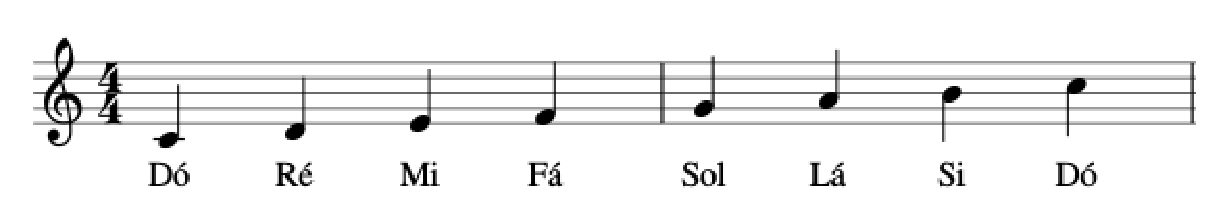
\includegraphics[scale=0.6]{figuras/escaladomaior.eps}
          \caption{Escala de Dó Maior}
          \label{escaladomaior}
        \end{figure}

        \begin{figure}[htb]
          \centering
          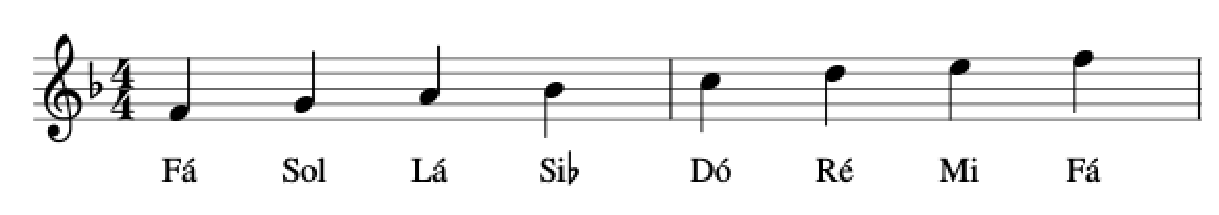
\includegraphics[scale=0.6]{figuras/escalafamaior.eps}
          \caption{Escala de Fá Maior}
          \label{escalafamaior}
        \end{figure}

      \subsubsection[Escalas Menores]{Escalas Menores}

        Assim como as escalas maiores, as escalas menores iniciam na tônica e possuem os seguintes intervalos, em tons, entre notas consecutivas: tom - semitom - tom - tom - semitom - um tom e meio - semitom. Classificando os intervalos, são: 2ªM - 2ªM - 2ªm - 2ªM - 2ªM - 2ªM - 2ªm. Nas Figuras \ref{escalalamenor} e \ref{escalamimenor}, estão representadas as escalas de Lá menor (que não possui nenhum acidente musical em sua armadura) e a de Mi menor (que possui um sustenido em Fá em sua armadura).

        \begin{figure}[htb]
          \centering
          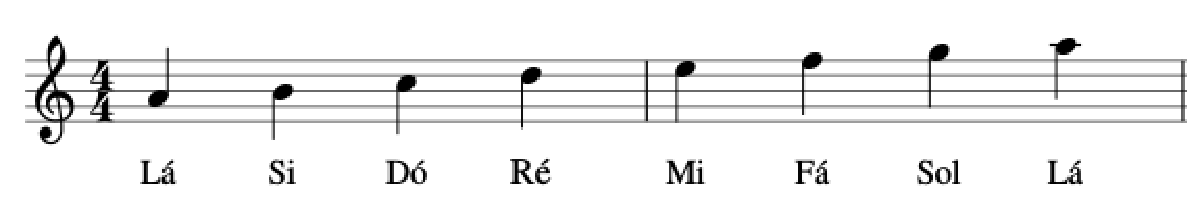
\includegraphics[scale=0.6]{figuras/escalalamenor.eps}
          \caption{Escala de Lá Menor}
          \label{escalalamenor}
        \end{figure}

        \begin{figure}[htb]
          \centering
          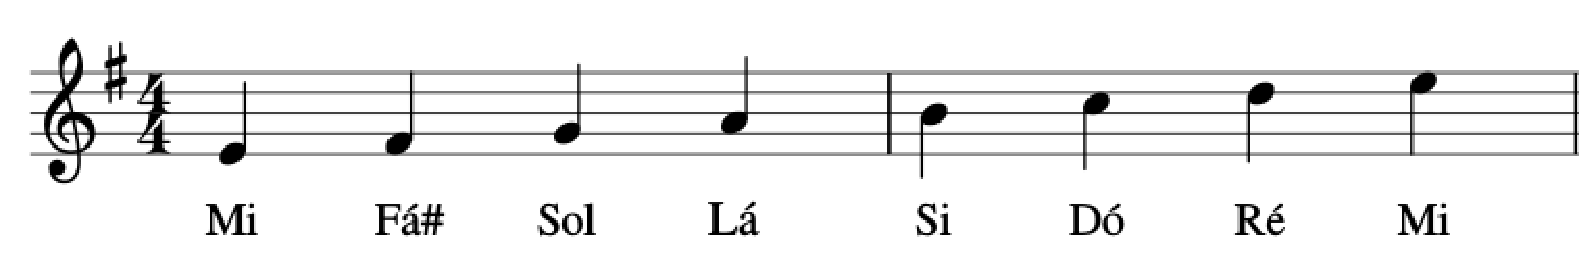
\includegraphics[scale=0.45]{figuras/escalamimenor.eps}
          \caption{Escala de Mi Menor}
          \label{escalamimenor}
        \end{figure}

        As escalas são utilizadas na composição de contrapontos definindo quais notas podem ser utilizadas para a geração do contraponto, de acordo com a escala da melodia principal.

    \subsection[Contraponto]{Contraponto}

      \citeonline{koellreuter} afirmam que contraponto é a arte de tornar independentes linhas melódicas de expressão autônoma, ou seja, combinar duas linhas melódicas simultâneas de forma que sejam melódicamente independentes, mas harmonicamente interdependentes. O objeto de estudo desse trabalho é o contraponto modal do século XVI, também chamado de contraponto palestriniano. Esse tipo de contraponto possui diversas espécies, cada uma definida pelo número de notas que um contraponto deve ter para cada nota da melodia principal (ou \textit{cantus firmus}). Nesse trabalho, serão tratados os contrapontos de primeira e segunda espécie (Figuras \ref{contrapontoprimeira} e \ref{contrapontosegunda}).

      \subsubsection[Contraponto de Primeira Espécie]{Contraponto de Primeira Espécie}

        Segundo \citeonline{jeppesen}, o contraponto de primeira espécie possui as seguintes regras:

        \begin{enumerate}
          \item deve haver uma nota no contraponto para cada nota do \textit{cantus firmus};
          \item os intervalos harmônicos entre o contraponto e o \textit{cantus firmus} devem ser consonates;
          \item deve-se começar e terminar em consonâncias perfeitas;
          \item se o contraponto for inferior (suas notas são mais graves que a do \textit{cantus firmus}), somente a oitava justa e o uníssono podem ser usados no início e no final;
          \item o uníssono só pode ocorrer no início ou no final;
          \item não é permitido oitavas e quintas paralelas (dois ou mais intervalos de oitavas ou de quintas seguidos);
          \item os intervalos não podem ser maiores que uma décima maior (10ªM);
          \item só são permitidos, no máximo, quatro intervalos seguidos de terças ou sextas (maiores ou menores) seguidos;
          \item se o movimento for paralelo, os intervalos melódicos devem ser menores que uma quarta ou um salto de oitava;
          \item deve-se priorizar movimento contrário (utilizar intervalo melódico ascendente se o \textit{cantus firmus} estiver em intervalo melódico descendente e vice-versa).
        \end{enumerate}

        \begin{figure}[htb]
          \centering
          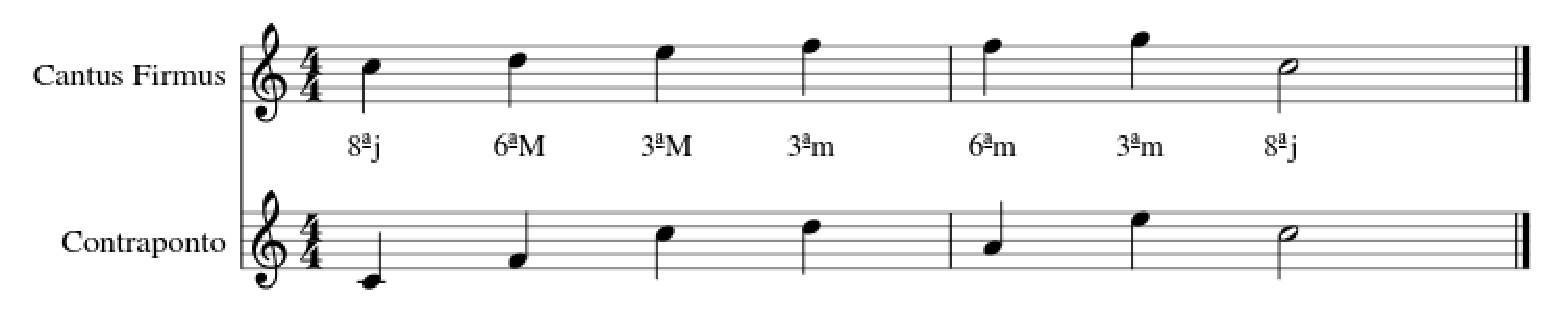
\includegraphics[scale=0.55]{figuras/contrapontoprimeira.eps}
          \caption{Exemplo de Contraponto de Primeira Espécie}
          \label{contrapontoprimeira}
        \end{figure}

      \subsubsection[Contraponto de Segunda Espécie]{Contraponto de Segunda Espécie}

        Segundo \citeonline{jeppesen}, o contraponto de segunda espécie possui, além das regras do contraponto de primeira espécie, as seguintes regras:

        \begin{enumerate}
          \item deve haver duas notas no contraponto para cada nota do \textit{cantus firmus};
          \item deve haver uma nota no contraponto para a última nota do \textit{cantus firmus};
          \item dissonâncias podem ser utilizadas em \textit{arsis} (porções não-acentuadas do compasso);
          \item as dissonâncias podem ser utilizadas apenas como nota de passagem, entre duas consonâncias e formando um grau conjunto, isto é, o intervalo melódico; entre a nota anterior e posterior à nota que provoca dissonância deve ser de segunda, maior ou menor;
          \item o uníssono só pode ser utilizado no início, final ou em \textit{arsis};
          \item se o uníssono for alcançado por salto (intervalo maior que uma segunda), deve ser deixado em grau conjunto na direção oposta à do salto;
          \item evitar quintas e oitavas em \textit{thesis} sucessivas, por se aproximarem de quintas e oitavas paralelas.
        \end{enumerate}

        \begin{figure}[htb]
          \centering
          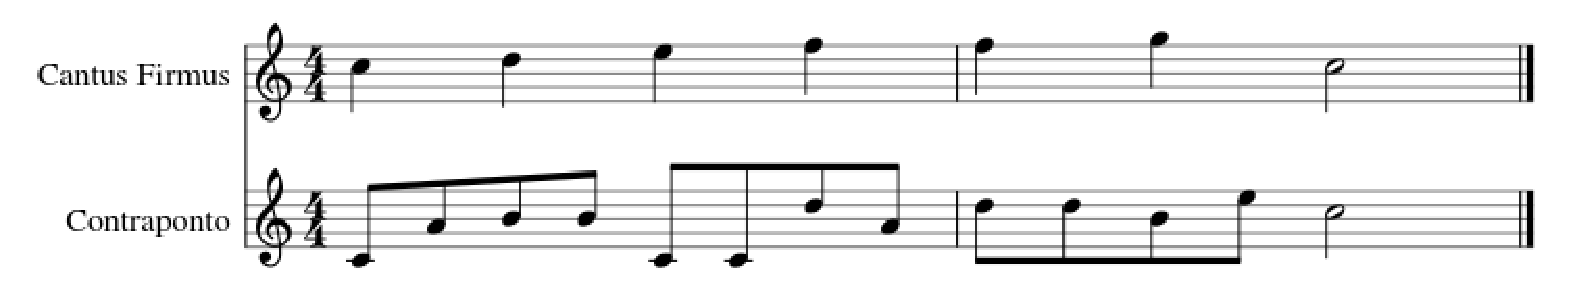
\includegraphics[scale=0.55]{figuras/contrapontosegunda.eps}
          \caption{Exemplo de Contraponto de Segunda Espécie}
          \label{contrapontosegunda}
        \end{figure}

      \subsubsection[Contraponto de Terceira Espécie]{Contraponto de Terceira Espécie}

        Segundo \citeonline{jeppesen}, o contraponto de segunda espécie possui, além das regras dos contraponto de primeira e segunda espécie, as seguintes regras:

        \begin{enumerate}
          \item deve haver quatro notas no contraponto para cada nota do \textit{cantus firmus};
          \item deve haver uma nota no contraponto para a última nota do \textit{cantus firmus};
          \item dissonâncias podem ser utilizadas em \textit{arsis} (porções não-acentuadas do compasso);
          \item as dissonâncias podem ser utilizadas como nota de passagem ou como notas auxiliares (bordaduras) inferiores - bordaduras são alcançadas e deixadas em grau conjunto, mas em direções opostas;
          \item As dissonâncias também podem ser empregadas por meio de \textit{cambiatas} - sequência de cinco notas com intervalos de segunda descendente, terça ascendente e segunda ascendente - que iniciem em semínimas acentuadas;
        \end{enumerate}

        FIGURA CONTRAPONTO TERCEIRA ESPECIE
        % \begin{figure}[htb]
        %   \centering
        %   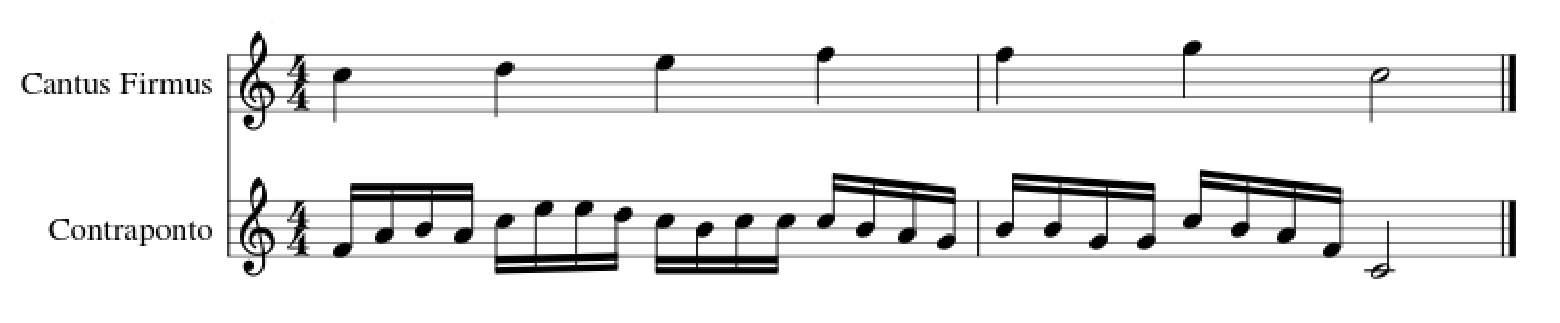
\includegraphics[scale=0.55]{figuras/contrapontoterceira.eps}
        %   \caption{Exemplo de Contraponto de Terceira Espécie}
        %   \label{contrapontoterceira}
        % \end{figure}

      \subsubsection[Contraponto de Quarta Espécie]{Contraponto de Quarta Espécie}

        Segundo \citeonline{jeppesen}, o contraponto de quarta espécie possui, além das regras dos contrapontos citados anteriormente, as seguintes regras:

        \begin{enumerate}
          \item deve haver duas notas no contraponto para cada nota do \textit{cantus firmus};
          \item dissonâncias devem ser utilizadas em \textit{thesis} (porções acentuadas do compasso) e vir ligadas das \textit{arsis} precedentes (síncope);
          \item consonâncias devem ser utilizadas em \textit{arsis} e resolver dissonâncias precedentes;
          \item as dissonâncias devem ser resolvidas seguindo as seguintes regras: se o contraponto for superior, devem ser utilizadas quartas e sétimas resolvidas em terças e sextas, respectivamente, se ele for inferior, devem ser utilizadas segundas e nonas resolvidas em terças e décimas, respectivamente;
          \item o uníssono pode ser utilizado livremente se estiver em cadeia de síncopes, se a cadeira for quebrada, deve seguir as regras previstas na segunda espécie;
        \end{enumerate}

        FIGURA CONTRAPONTO QUARTA ESPECIE
        % \begin{figure}[htb]
        %   \centering
        %   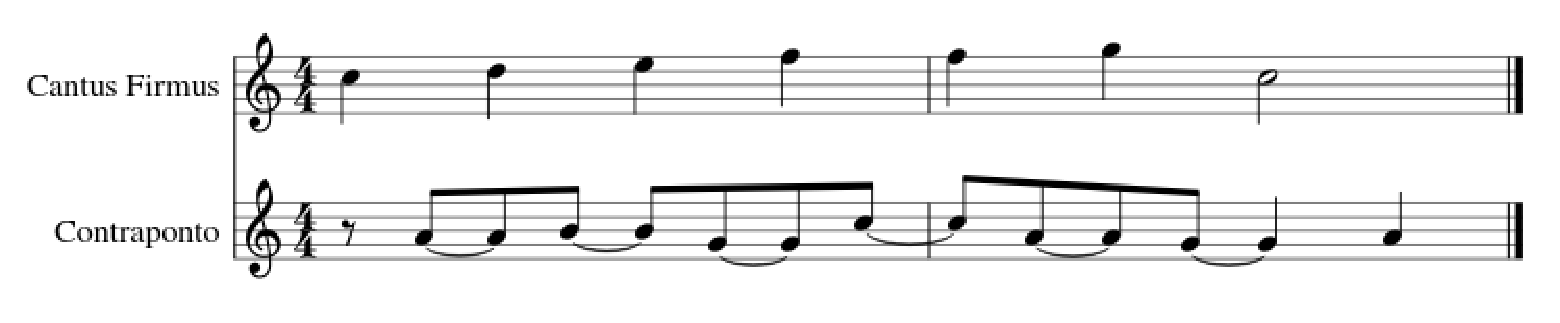
\includegraphics[scale=0.55]{figuras/contrapontoquarta.eps}
        %   \caption{Exemplo de Contraponto de Quarta Espécie}
        %   \label{contrapontoquarta}
        % \end{figure}

  \section[Grafos]{Grafos}

    Na geração de um contraponto, cada nota dele depende da nota dos \textit{cantus firmus} tocada em simultâneo devido a regras definidas com base no intervalo harmônico -- como a proibição de intervalos dissonantes, por exemplo. Porém, as notas disponíveis para um dado tempo do contraponto também depende das notas anteriores a ela devido a regras relacionadas à intervalos melódicos e repetição ou uso demasiado de intervalos harmônicos repetidos -- como a proibição de oitavas paralelas. Sendo assim, a nota atual define, em conjunto com a próxima nota do \textit{cantus firmus}, quais notas podem ser empregadas no próximo tempo. Dada tal organização, essa estrutura pode ser representada por um grafo.

    Grafo é uma estrutura formada por vértices (os nós que representam a unidade fundamental da estrutura) e arestas (ligações que indicam quais outros vértices podem ser alcançados a partir de um). Na Figura \ref{grafonotas} está representado um exemplo de estrutura formada pelas notas possíveis em um contraponto. Vale ressaltar que, segundo \citeonline{halim}, como a estrutura do contraponto não é diretamente representada por um grafo na solução proposta, ela é definida como um grafo implícito.

    \begin{figure}[htb]
      \centering
      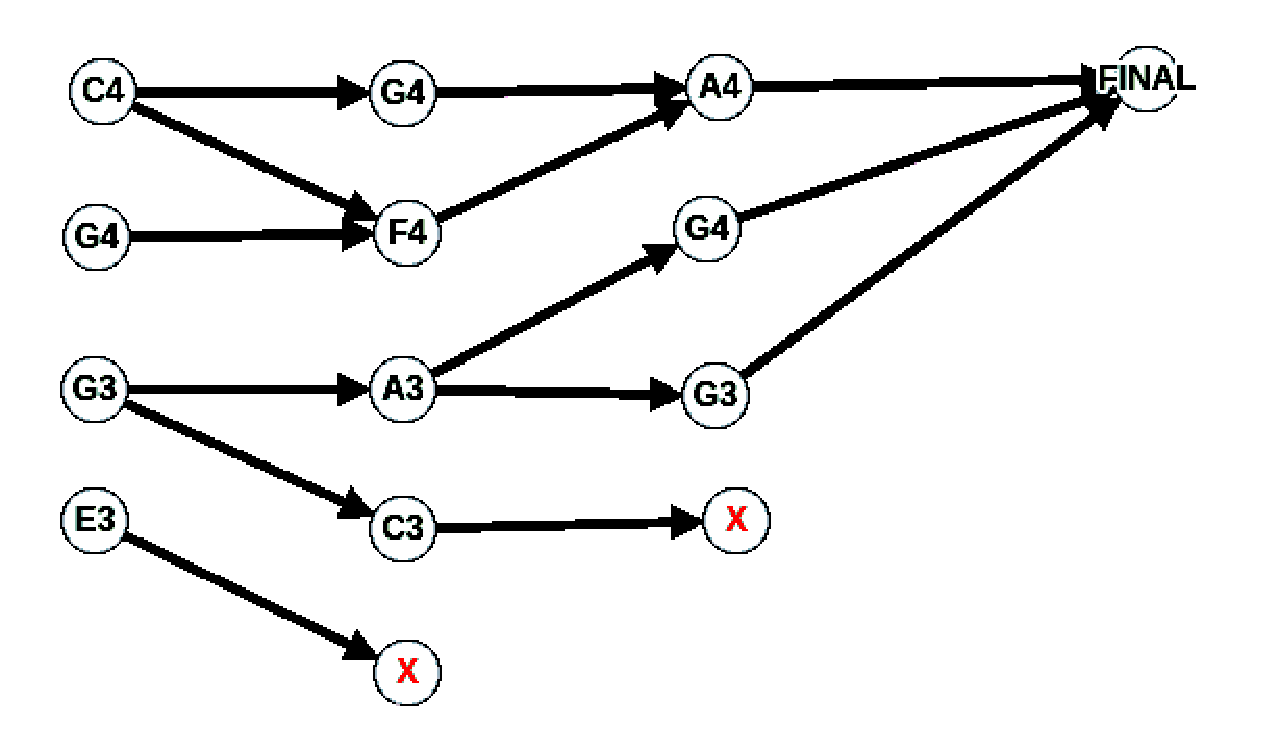
\includegraphics[scale=0.55]{figuras/grafonotas.eps}
      \caption{Exemplo de Notas Possíveis Representados em Grafo}
      \label{grafonotas}
    \end{figure}

    \subsection[Grafos Direcionados Acíclicos]{Grafos Direcionados Acíclicos}

      Um grafo pode possui diversas classificações. Uma classificação clássica é quanto à sua direção. Se as arestas de um grafo não definem a direção da ligação, isto é, se os vértices X e Y estão ligados por uma aresta, significa que X é diretamente alcançável (apenas um vértice é necessário para navegar da origem ao destino) a partir de Y e Y é diretamente alcançável a partir de X, esse grafo é classificado como não-direcionado. Mas se as arestas possuem direção e X ser diretamente alcançável por Y não garante que Y é diretamente alcançável a partir de X, esse grafo é direcionado, como afirma \citeonline{halim}. Veja a Figura \ref{nodirxdir}.

      \begin{figure}[htb]
        \centering
        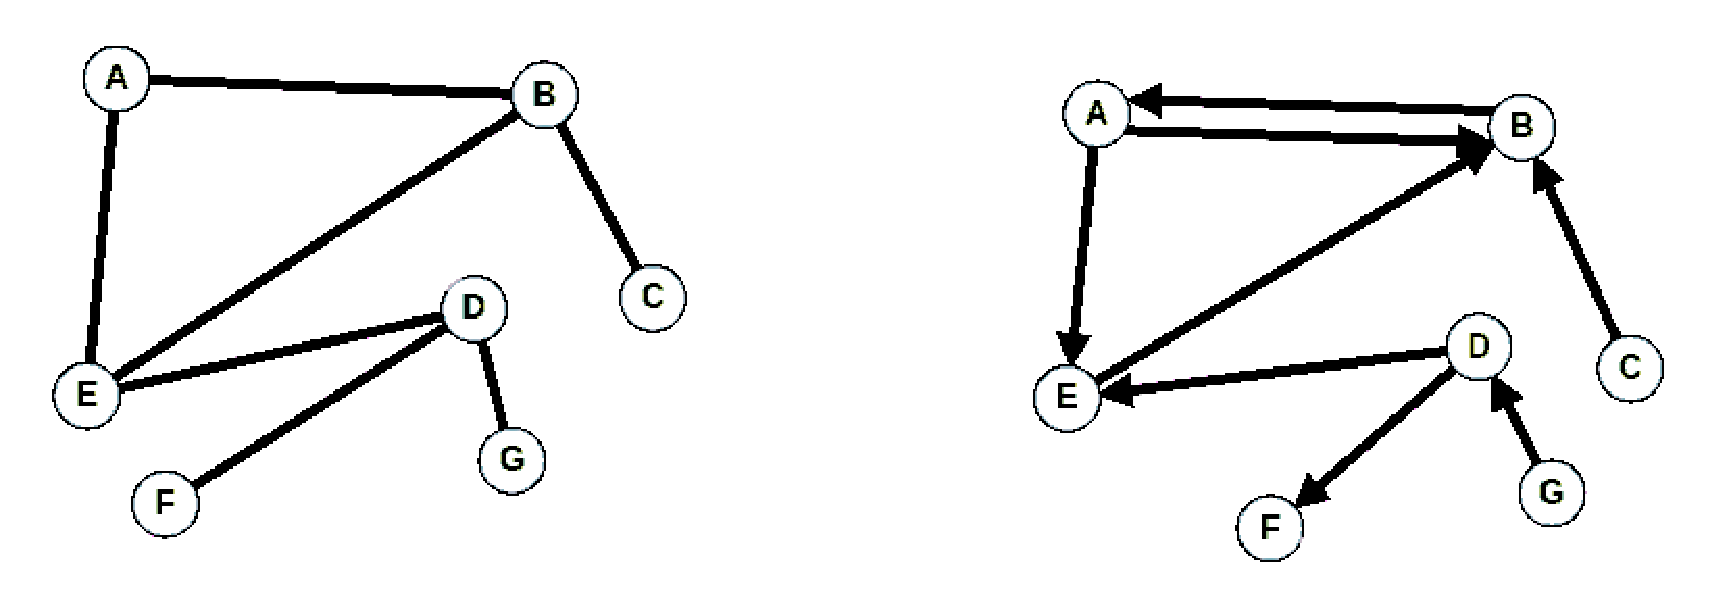
\includegraphics[scale=0.47]{figuras/nodirxdir.eps}
        \caption{Exemplos de Grafo Não-Direcionado e Direcionado}
        \label{nodirxdir}
      \end{figure}

      Grafos direcionados podem ser classificados como cíclicos ou acíclicos. Grafos acíclicos são grafos que não possuem ciclos, isto é, para todo vértice A, se A alcança B, B não alcança A. Se para pelo menos um par de vértices A e B, A alcançar B e B alcançar A, esse grafo é considerado cíclico.

      Dadas tais definições, é possível perceber que a estrutura do contraponto é um grafo direcionado acíclico (ou DAG, sigla para \textit{Direct Acyclic Graph}). Nesse tipo de grafo, cada vértice possui um ou mais pais -- vértices que apontam para ele. Assemelhando-se à estrutura de uma árvore (grafo com raiz definida como o único vértice sem pai e que cada outro vértice tem apenas um pai), o DAG difere-se por cada vértice por ter mais de um pai e vários vértices sem pai, mas mantém a propriedade de ser navegável em apenas uma direção, impedindo a formação de \textit{loops} que tornariam a exploração da solução um processo infinito. A Figura \ref{naodagdagarvore} exemplifica esses três tipos de grafos.

      \begin{figure}[htb]
        \centering
        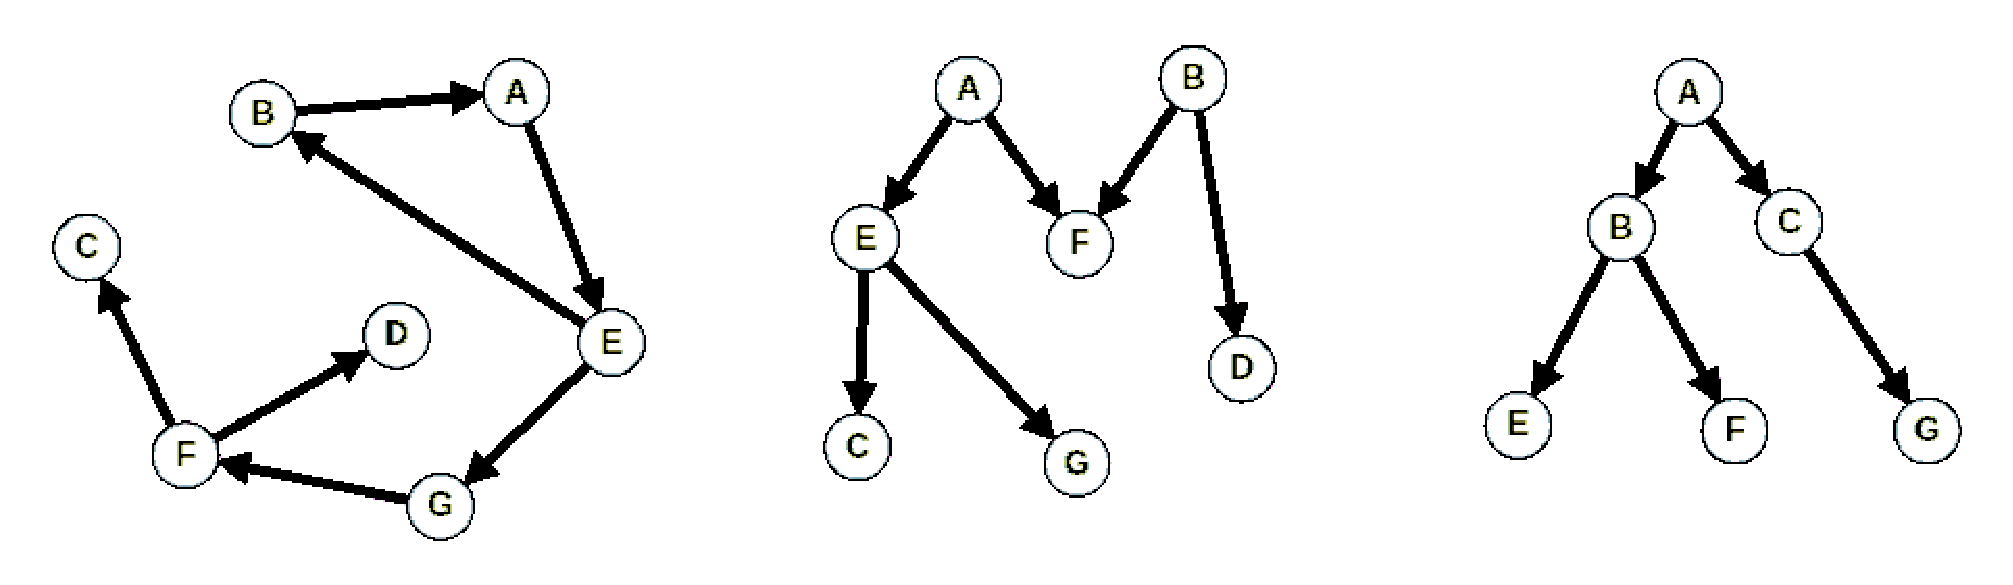
\includegraphics[scale=0.47]{figuras/naodagdagarvore.eps}
        \caption{Exemplos de Grafo Não-DAG, DAG e Árvore}
        \label{naodagdagarvore}
      \end{figure}

    \subsection[Travessia de Grafos]{Travessia de Grafos}

      Há diversas formas de se visitar todos os vértices de um grafo. O número total de formas é igual ao fatorial do número de vértices, pois uma travessia difere-se de outra apenas pela ordem em que os vértices são visitados. Contudo, algumas travessias possuem propriedades específicas e utilizam as arestas para definí-las. As duas travessias mais conhecidas são a busca por profundidade (DFS, sigla para \textit{Depth-First Search}) e a busca por largura (BFS, sigla para \textit{Breadth-First Search}).

      A busca por profundidade funciona de forma recursiva. Primeiramente, um vértice é escolhido como o vértice inicial, antes de explorá-lo (analisar o valor contido no vértice), visitamos todos as suas conexões, para cada vértice conectado, antes de explorá-lo, visitamos sua conexões. Esse processo de visita ocorre até atingir um vértice que não possui arestas ou possui apenas conexões já visitadas. Ao chegar nesse ponto, o algoritmo explora, recursivamente, os vértices previamente visitados. Utilizando uma estrutura de dados conhecida, uma DFS pode ser implementada por meio do uso de pilhas, devido à propriedade delas que definem que o último a entrar na estrutura é o primeiro a sair. Veja a Figura \ref{dfs}.

      \begin{figure}[htb]
        \centering
        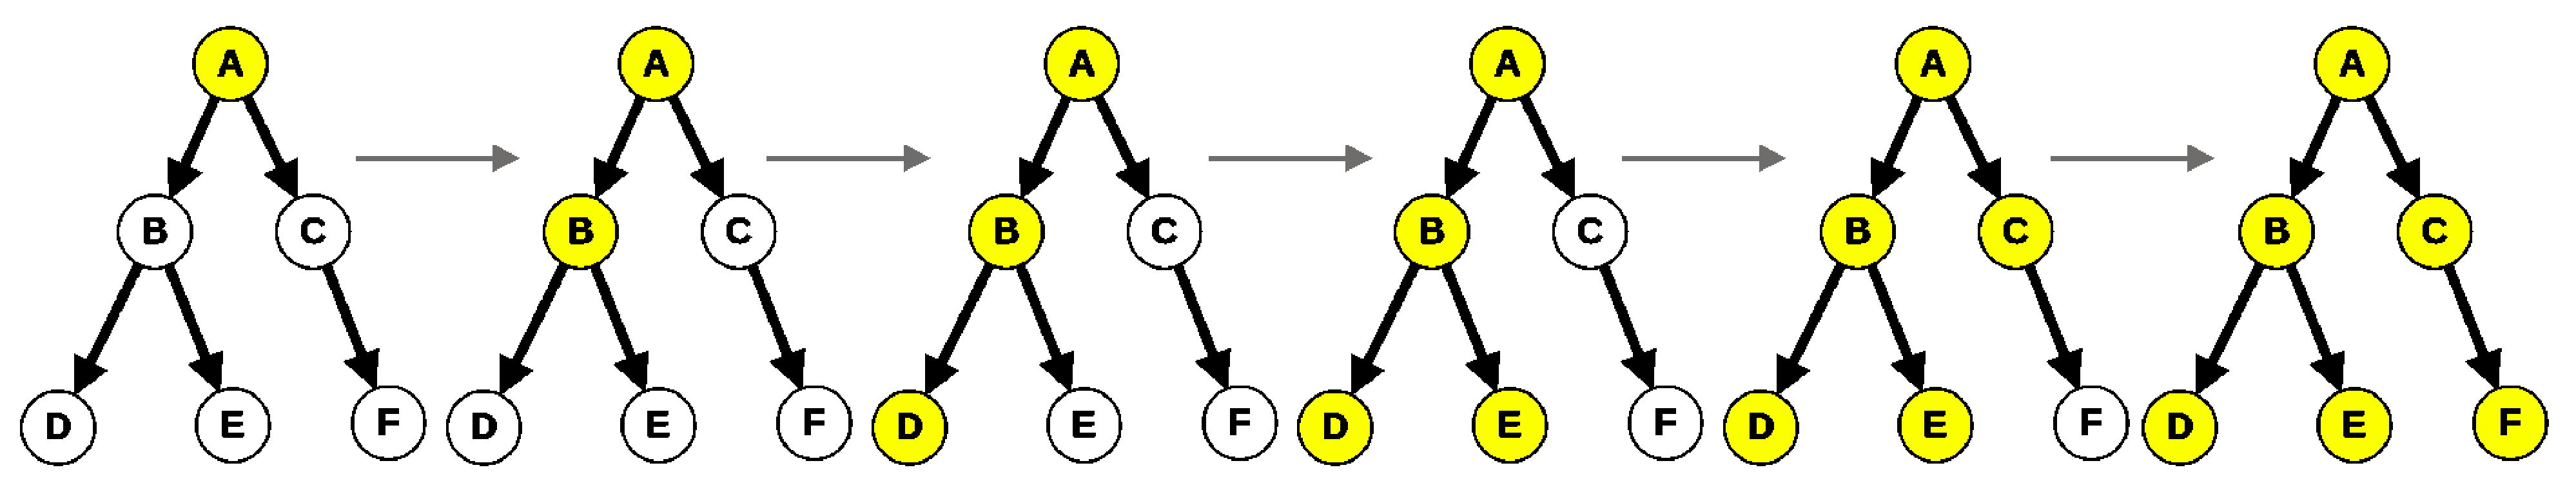
\includegraphics[scale=0.25]{figuras/dfs.eps}
        \caption{Exemplo de DFS}
        \label{dfs}
      \end{figure}


      A busca por largura inicia em um vértice e visita todos os filhos (vértices para os quais o vértice atual aponta) antes de visitar os filhos destes. Desse modo, em um DAG, o primeiro nível (composto por vértices sem pai) é completamente visitado antes de o segundo nível (filhos destes) ser visitado e assim sucessivamente. Utilizando uma estrutura de dados conhecida, uma BFS pode ser implementado por meio do uso de filas devida à propriedade delas que define que o primeiro a entrar na estrutura é o primeiro a sair. Veja a Figura \ref{bfs}.

      \begin{figure}[htb]
        \centering
        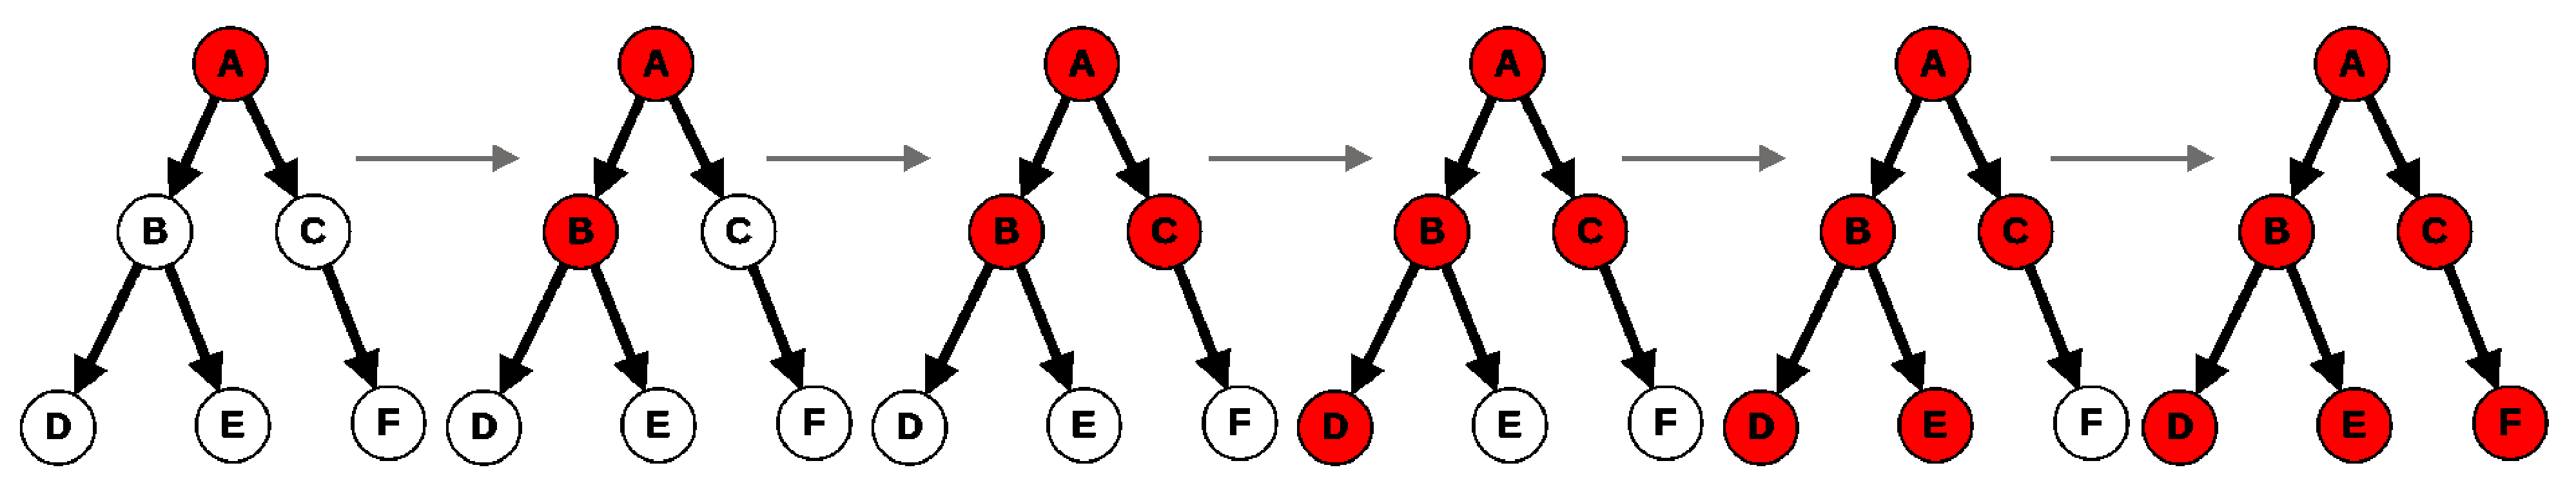
\includegraphics[scale=0.25]{figuras/bfs.eps}
        \caption{Exemplo de BFS}
        \label{bfs}
      \end{figure}

      Para a solução proposta nesse trabalho será usada a DFS por dois motivos. O primeiro é que a DFS chega a uma folha (vértice sem filhos) primeiro, o que é interessante para a solução pois busca-se a primeira solução disponível. O segundo motivo é que a DFS permite que seja utilizado um único vetor, inserindo e retirando no final deste (consequentemente, funcionando de forma análoga a uma pilha), economizando memória e diminuindo o tempo de execução que levaria para fazer cópias do vetor em uma BFS, pois o comportamento análogo a uma fila exigiria isso.


  \section[Paradigmas de Solução de Problema]{Paradigmas de Solução de Problema}

    O objetivo de encontrar uma sequência de notas que se encaixe nas regras do contraponto pode ser alcançado pela análise de todas as combinações de notas possíveis, verificando se cada uma delas atende às regras e retornando como resposta a primeira sequência que atender. A esse tipo de busca pela solução se dá o nome de Busca Completa.

    \subsection[Busca Completa]{Busca Completa}

      \citeonline{halim} afirma que na Busca Completa, todo ou parte do espaço de soluções possíveis é explorado. No código \ref{codecs} é possível observar a geração de todas as combinações de notas possíveis para um contraponto por meio de um algoritmo de \textit{backtracking} (algoritmo recursivo de busca completa). Contudo, nesse caso, tal abordagem possui alta complexidade em termos de execução. Suponhando um espaço amostral com 88 notas disponíveis e um \textit{cantus firmus} com 50 notas, apenas para o contraponto de primeira espécie há $88^{50}$ sequências possíveis.

      \begin{lstlisting}[language={C}, caption={Busca Completa}, label={codecs}]
      // Vector with 88 musicais notes found on piano
      vector<Note> available_notes(88);

      void backtracking(vector<Note> counterpoint) {
        // Process solution if
        // counterpoint candidate and cantus firmus
        // has the same number of notes
        if(counterpoint.size() == CANTUS_FIRMUS_SIZE){
          process_solution(counterpoint);
        }

        // Append each available note to counterpoint
        for(int i = 0; i < (int) available_notes.size(); i++){
          counterpoint.push_back(available_notes[i]);
          backtracking(counterpoint);
          counterpoint.pop_back();
        }
      }
      \end{lstlisting}

      Para diminuir a complexidade de uma busca completa, podas podem ser aplicadas. Podas são aplicadas quando uma parte gerada da solução já indica que ela certamente não gerará uma solução. No caso do contraponto, por exemplo, podemos podar soluções parciais que já apresentem um número de movimentos reversos maior que o definido pelas regras mesmo antes de chegarem à última nota.

    \subsection[Programação Dinâmica]{Programação Dinâmica}

      Mesmo após a aplicações de todas as podas possíveis, ainda há o caso de diversos estados serem recalculados. Como explicado anteriormente, uma nota em nosso grafo pode ter mais de um pai, isto é, mais de uma nota pode ter a nota atual como a seguinte em uma possível solução. Entretanto, uma vez alcançada a nota atual, o resto da solução é o mesmo, sendo redundante calcular esse estado (e se ele levará a possíveis soluções ou não) mais de uma vez. Tendo estados que se repetem entre soluções, é possível aplicar um paradigma de solução de problemas chamado Programação Dinâmica.

      A Programação Dinâmica (ou DP, sigla para \textit{Dynamic Programming}) é um paradigma de solução de problema baseado em estados, transições e casos-base, segundo \citeonline{halim}. Cada estado resolve um problema e para isso ele precisa resolver subproblemas. A forma como o estado atual se relaciona com seus subestados é denominada transição.

      Dada a forma recursiva como a DP funciona, casos-base garantem que o algoritmo não assuma uma forma infinita. Esses casos são aqueles com solução trivial que não necessita da resolução de subproblemas para respondê-la. A ideia central da DP é que subproblemas se repetem durante a solução, portanto, um estado já calculado deve ter seu resultado armazenado para futuras consultas que provavelmente acontecerão durante a resolução do problema.

      Um exemplo clássico de como uma DP pode agilizar a resolução de um problema com subestados repetidos é o cálculo da sequência de Fibonacci. Os números da sequência de Fibonacci seguem a seguinte regra:

      \[ F(n) = \left\{ \begin{array}{ll}
         n & \mbox{se $n \leqslant 1$}\\
        F(n-1) + F(n-2) & \mbox{c.c.}\end{array} \right. \]

      No cálculo dos números de Fibonacci, o estado em uma dada posição N é o valor do N-ésimo número de Fibonacci. Para calculá-lo, utiliza-se os dois números de Fibonacci anteriores a ele na sequência, sendo essa a transição do algoritmo. Os únicos dois casos em que o cálculo não necessita dos dois anteriores são os números de Fibonacci nas posições 0 e 1, para esses, a solução é, por definição, 0 e 1, respectivamente. Dessa forma, 0 e 1 são nossos casos-base.

      Tomando como exemplo o cálculo de F(5), calculando-o sem memorização de estados, é necessário calcular F(4) e F(3). Para calcular o F(4), é preciso calcular o F(3) e o F(2). Sem a memorização, após o cálculo do F(4), o F(3), que já havia sido calculado para o F(4), será recalculado, bem como o F(2) para o cálculo do F(3). Contudo, se o valor de F(3) for memorizado em alguma estrutura de dados (geralmente um vetor) para consultas futuras, seria necessário calcular cada estado apenas uma vez. Na figura \ref{nodpxdp} há um comparativo entre a árvore de chamadas para F(5) com e sem a memorização característica de uma DP, os nós em amarelo representam os nós que utilizam recursão, os nós vermelhos são os casos-base e os nós verdes utilizam valores previamente memorizados.

      \begin{figure}[htb]
        \centering
        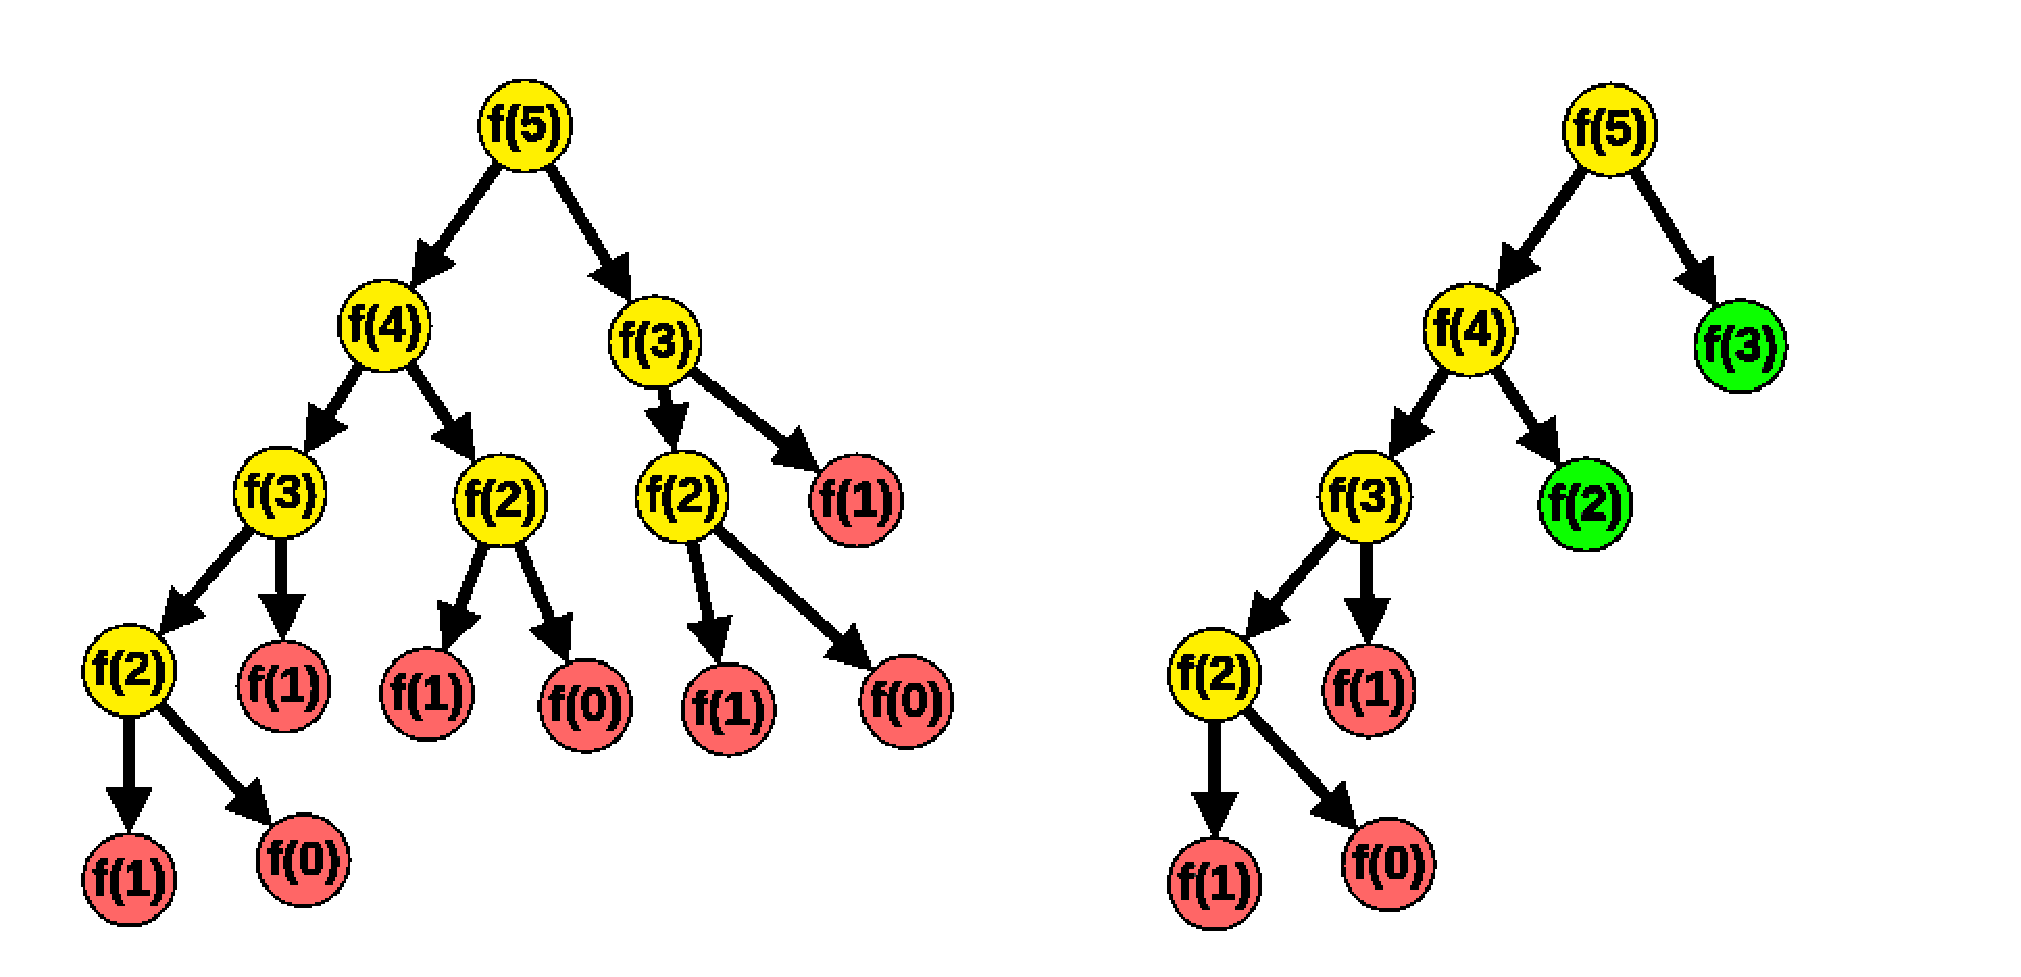
\includegraphics[scale=0.5]{figuras/nodpxdp.eps}
        \caption{Comparativo entre a abordagem não-DP e DP para o cálculo do F(5)}
        \label{nodpxdp}
      \end{figure}

      Neste trabalho, a DP será utilizada para a geração do contraponto. O estado sendo caracterizado por uma dada nota em uma dada posição no contraponto com um número específico de movimentos paralelos e terças e sextas paralelas. A transição é definida pela solução da próxima nota no contraponto, partindo da nota atual. O caso-base é definido por quando o algoritmo atinge o final do \textit{cantus firmus}, retornando que aquela solução é válida, já que não foi podada nenhuma vez durante a construção daquela solução.
